\section{Resultados}

En esta sección vamos a analizar y comentar los resultados de la batería experimental que hemos propuesto. En base a ellos responderemos a las cuestiones que nos habíamos planteado al principio del trabajo. Dividiremos por tanto esta sección en cinco subsecciones, donde en la primera se analizarán de manera genérica los resultados y en las siguientes se responderá directamente a las cuestiones planteadas en la introducción. Se mostrarán solo las gráficas o los resultados pertinentes, mientras que el resto puede encontrarse en el mismo código. Al referirnos a un modelo entrenado por un algoritmo concreto, nos referiremos y usaremos el mejor modelo obtenido durante ese proceso de entrenamiento, en términos del que obtenga menor error de validación. 

A excepción de la cuestión \textit{P3}, en el resto de comparativas valorares solamente el rendimiento del modelo en la tarea correspondiente y no los recursos computacionales necesarios para llevarla a cabo. Los resultados completos del entrenamiento pueden encontrarse en los apéndices \ref{sec:apendiceA} y \ref{sec:apendiceB}, que contienen las tablas referentes al rendimiento y el tiempo de entrenamiento, respectivamente.

\subsection{Comentarios generales}

Antes de empezar a responder las preguntas que nos hicimos en \ref{sec:objinf}, tomaremos una idea general de los resultados del entrenamiento. Seleccionaremos seis gráficas que resultan representativas, res del entrenamiento de modelos con metaheurísticas y otras tres con optimizadores. La afirmación más inmediata, que confirman todos los resultados, es algo que ya sabíamos por la literatura: las metaheurísticas tienen un rendimiento inferior al de los optimizadores. Aunque hay casos, como vemos en la figura \ref{fig:resgen1}, donde su rendimiento es muy similar en cuanto al error de generalización y el valor de \textit{accuracy}, y en el que las metaheurísticas minimizan más la función de pérdida. Estos casos son siempre para conjuntos de datos pequeños con poca complejidad en la tarea y usando modelos con pocos parámetros. 

\begin{figure}[!tbp]
  \centering
  \subfloat{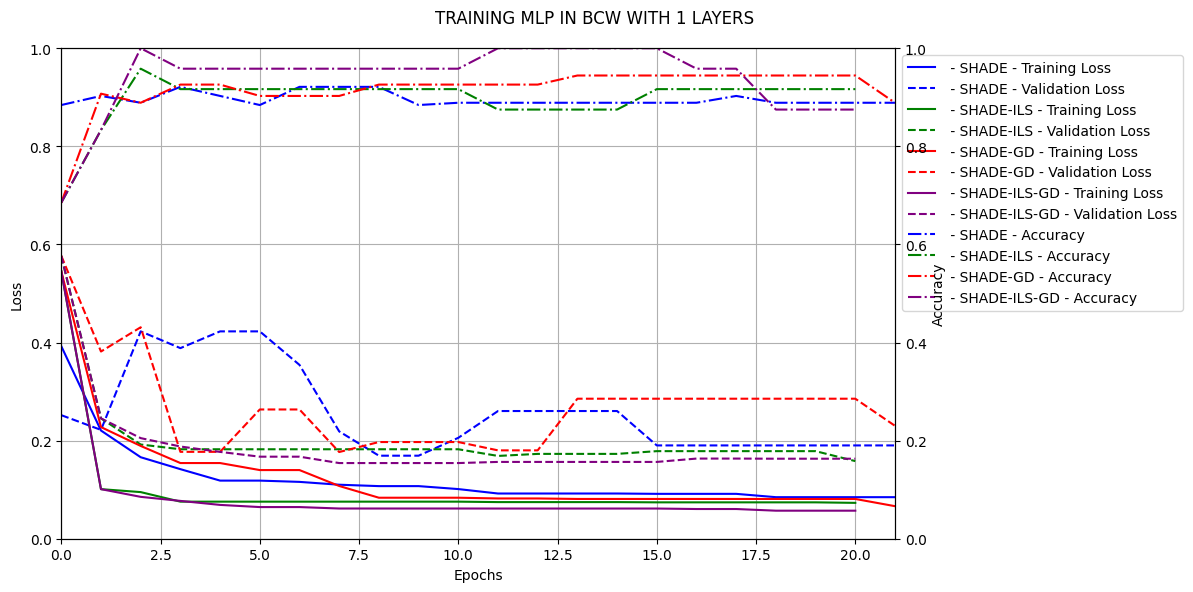
\includegraphics[width=0.5\textwidth]{Plantilla_TFG_latex//imagenes//Inf//Resultados/bcw_1layer_mh.png}}
  \hfill
  \subfloat{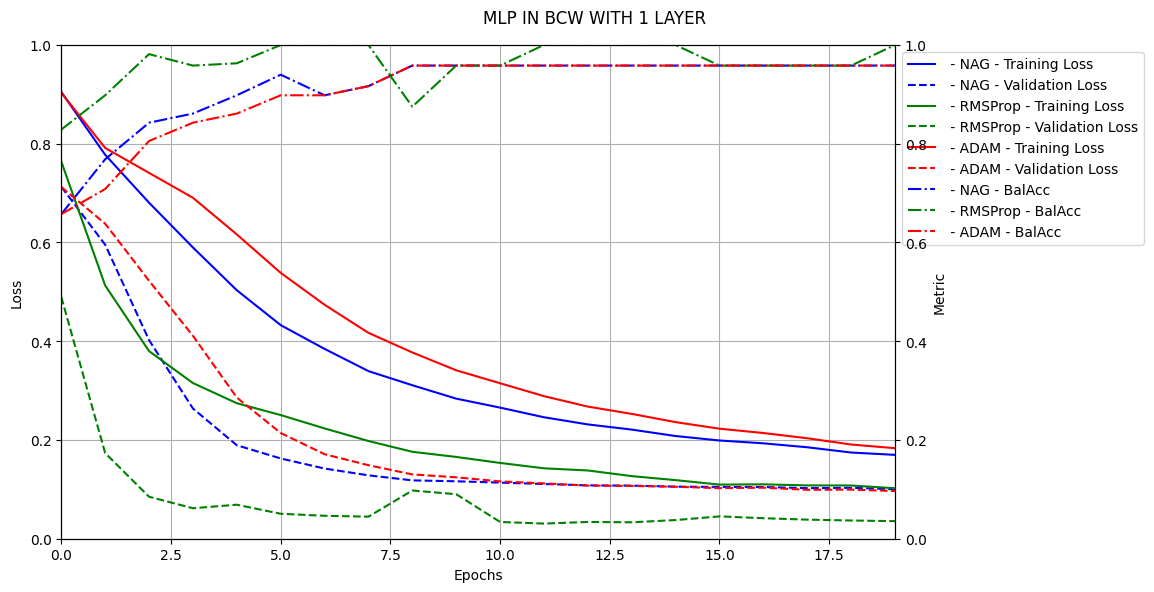
\includegraphics[width=0.48\textwidth]{Plantilla_TFG_latex//imagenes//Inf//Resultados/bcw_1layer_gd.png}}
  \caption{Resultados del entrenamiento sobre el conjunto de datos BCW, entrenando un modelo MLP de 1 capa a través de técnicas metaheurísticas (izquierda) y optimizadores basados en gradiente descendente (derecha).}
\label{fig:resgen1}
\end{figure}


\begin{figure}[!tbp]
\label{fig:resgen2}
  \centering
  \subfloat{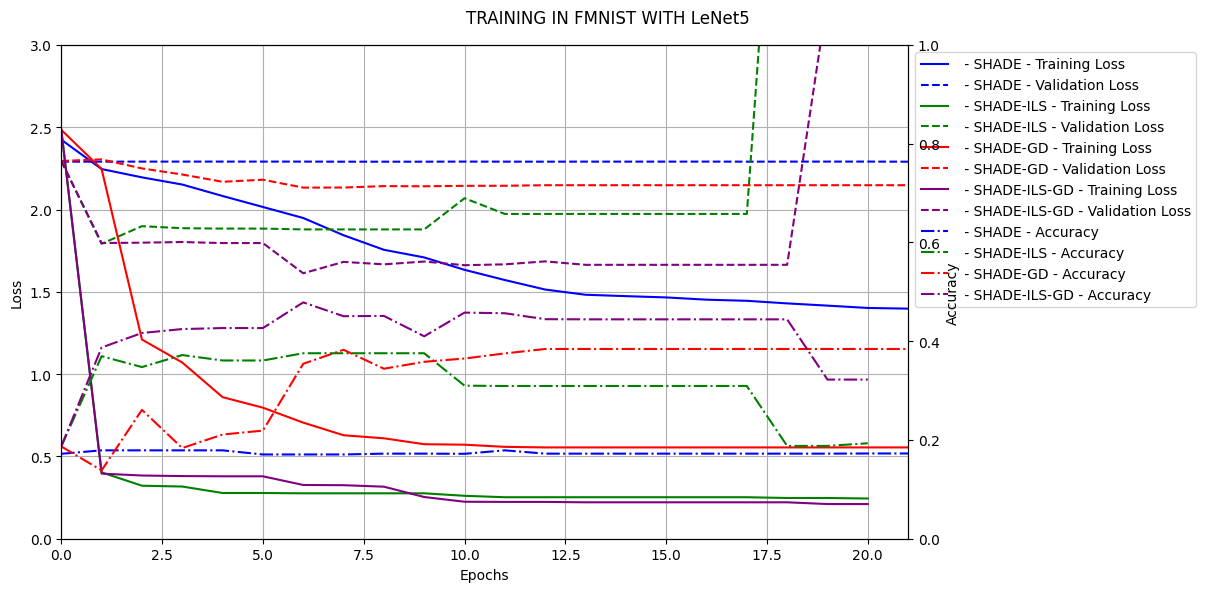
\includegraphics[width=0.5\textwidth]{Plantilla_TFG_latex//imagenes//Inf//Resultados/fmnist_lenet5_mh.png}}
  \hfill
  \subfloat{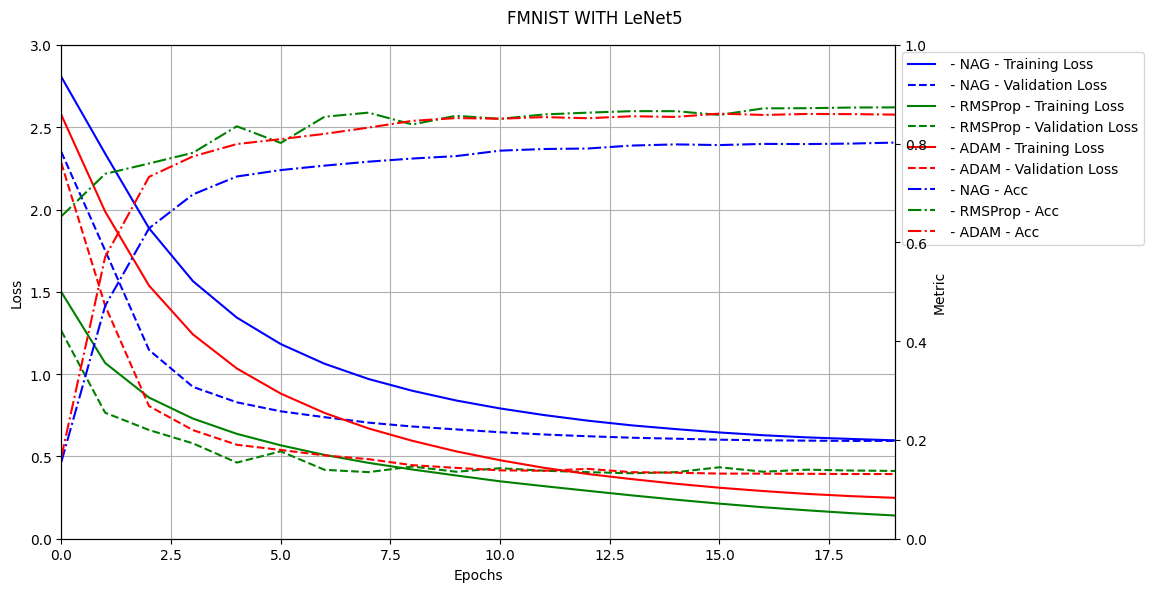
\includegraphics[width=0.48\textwidth]{Plantilla_TFG_latex//imagenes//Inf//Resultados/fmnist_lenet5_gd.png}}
  \caption{Resultados del entrenamiento sobre el conjunto de datos F-MNIST, entrenando el modelo LeNet5 a través de técnicas metaheurísticas (izquierda) y optimizadores basados en gradiente descendente (derecha).}
\end{figure}


\begin{figure}[!tbp]
\label{fig:resgen3}
  \centering
  \subfloat{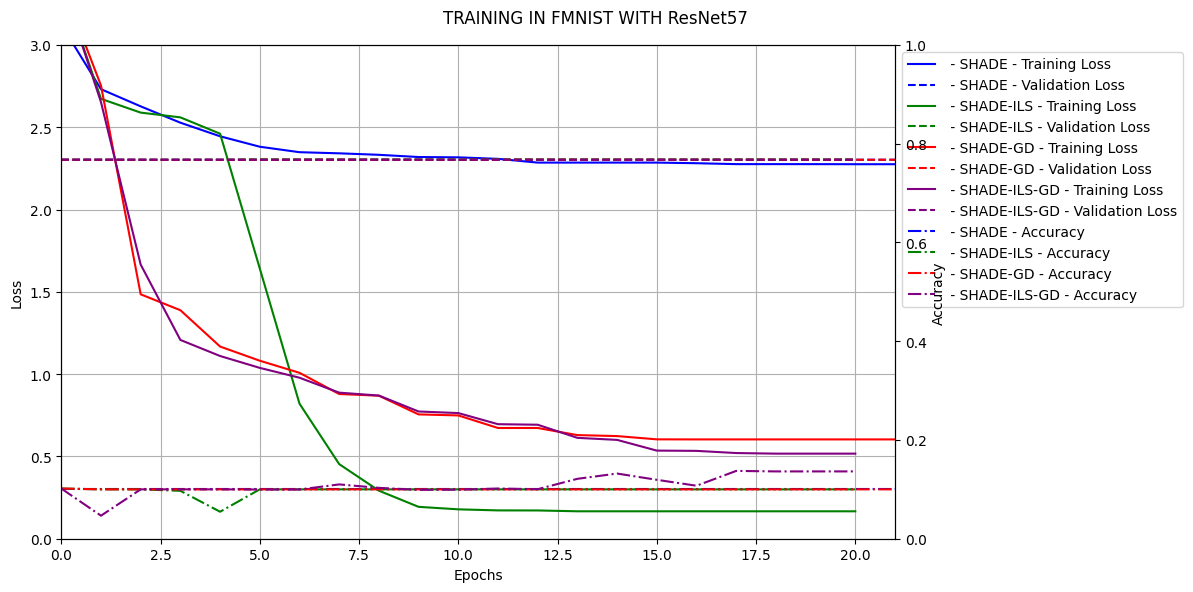
\includegraphics[width=0.5\textwidth]{Plantilla_TFG_latex//imagenes//Inf//Resultados/fmnist_resnet57_mh.png}}
  \hfill
  \subfloat{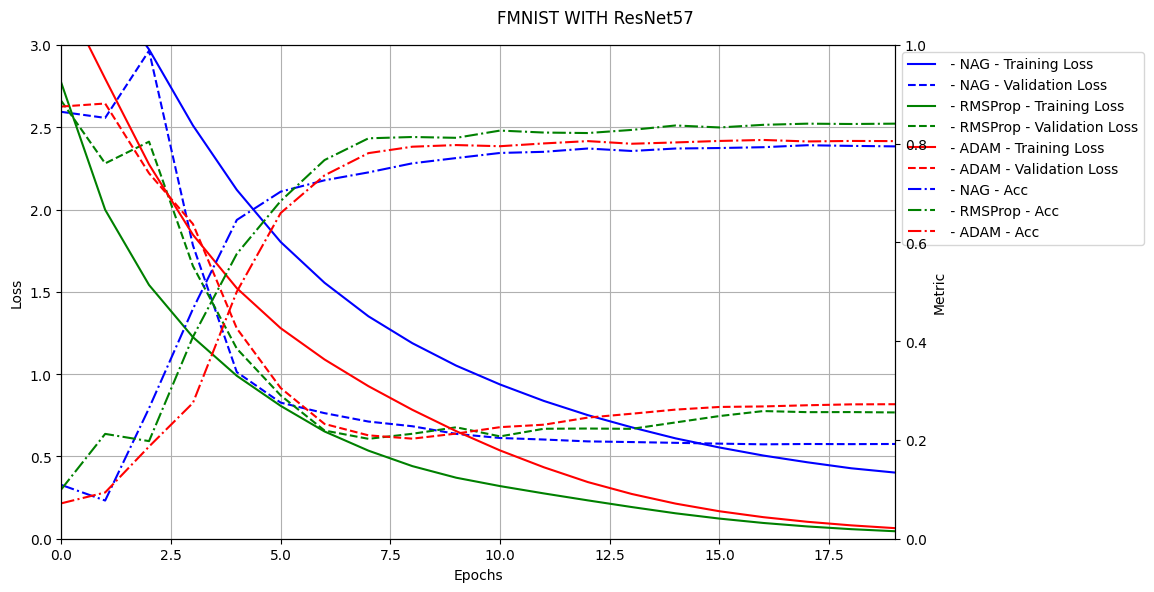
\includegraphics[width=0.48\textwidth]{Plantilla_TFG_latex//imagenes//Inf//Resultados/fmnist_resnet57_gd.png}}
  \caption{Resultados del entrenamiento sobre el conjunto de datos F-MNIST, entrenando el modelo ResNet57 a través de técnicas metaheurísticas (izquierda) y optimizadores basados en gradiente descendente (derecha).}
\end{figure}


Así, por ejemplo, cuando aumentamos un poco la cantidad de datos y la dificultad de la tarea vemos en la figura \ref{fig:resgen2} que el rendimiento empeora considerablemente. Aquí, el error de entrenamiento sigue minimizándose al mismo nivel que lo hacen las técnicas basadas en gradiente descendente, pero vemos que a lo largo del entrenamiento el error de generalización aumenta de manera significativa. Si además aumentamos el número de parámetros del modelo que entrenamos, como vemos en la figura \ref{fig:resgen3}, donde usamos el mismo conjunto de datos pero con un modelo aproximadamente tres veces más grandes, los resultados tienden a acercarse al de un clasificador aleatorio. En este caso, el error de generalización se mantiene estable, lo que indica que estos algoritmos de aprendizaje no consiguen mejorar nada a lo largo de todo el entrenamiento. No podemos afirmar que no mejore al modelo original, con parámetros aleatorios según la inicialización de Glorot, ya que el primer valor del entrenamiento se guarda justo después de entrenar y no antes, por lo que no se muestra en la gráfica el rendimiento del mejor modelo original de la población y podría darse el caso de que se realice una mejora únicamente en la primera iteración.

Cabe resaltar también, como se observa en las figuras mencionadas, que las técnicas metaheurísticas son muy efectivas minimizando el error de la función de pérdida, logrando en este aspecto mejores resultados que el gradiente descendente en algunos casos, pero muy deficientes generalizando ese error. Este último error es el que nos interesa realmente. Por lo tanto, y confirmando la literatura existente al respecto, concluimos que las metaheurísticas no son actualmente una alternativa a los algoritmos de aprendizaje basados en gradiente descendente. Más aún si tenemos en cuenta la enorme diferencia de tiempo que hay en el entrenamiento de cada uno.

Hacemos una mención especial al único caso de la experimentación en el que un modelo entrenado a través de metaheurísticas ha sido capaz de mejorar a los optimizadores clásicos: en la tarea de regresión en el conjunto de datos BHP, entrenando con SHADE-ILS-GD al modelo MLP con una capa, se logró un error de entrenamiento de 8.9, un error de generalización de 4.64 y una puntuación R$^2$ de 0.84. RMSProp es el optimizador que mejor rendimiento consigue con unos valores de 61.7, 4.67 y 0.82, respectivamente.

Las diferencias que observamos en los resultados con respecto a los obtenidos en \cite{MHtrainingClase} pueden deberse a tres factores principales:

\begin{itemize}

\item Diferencias en los hiperparámetros usados.

\item Diferencias en la implementación de las técnicas metaheurísticas

\item Menor cantidad de recursos computacionales dedicados al entrenamiento con las técnicas metaheurísticas.

\end{itemize}

\subsection{Cuestión P1}


Ahora sí empezaremos a responder en orden a las cuestiones planteadas. Primero veremos qué factores influyen más en el rendimiento de las técnicas metaheurísticas. Elegimos solo tareas de clasificación para que la comparación sea más sencilla. Compararemos los resultados de las tareas que se muestran en la tabla \ref{tab:expP1} en base a tres criterios: número de parámetros del modelo, complejidad de la tarea y tamaño del conjunto de datos.

\begin{table}[]
\centering
\begin{tabular}{|c|c|c|}
\hline
\textbf{Conjunto de datos} & \textbf{Complejidad} & \textbf{Cantidad de datos} \\ \hline
\textbf{BCW}               & Fácil                & Poca                       \\ \hline
\textbf{MNIST}             & Fácil                & Mucha                      \\ \hline
\textbf{WQ}      & Media                & Intermedia                 \\ \hline
\textbf{F-MNIST}           & Media                & Mucha                      \\ \hline
\textbf{CIFAR-10-G}             & Media-alta           & Mucha                      \\ \hline
\end{tabular}
\caption{Tareas a comparar para responder a la cuestión P1.}
\label{tab:expP1}
\end{table}

Analizando las tablas de los resultados de los entrenamientos separados por tarea, podemos sacar algunas nociones generales. Como esperábamos, a medida que aumentamos la complejidad de la tarea, la cantidad de ejemplos y el número de parámetros del modelo, peor es el rendimiento que tienen las técnicas metaheurísticas. Cuando la cantidad de datos es pequeña y la tarea es fácil, estas técnicas obtienen un rendimiento similar al que obtienen los optimizadores basados en gradiente descendente, aunque siempre por debajo. En muchos casos consiguen minimizar más la función de pérdida, pero luego obtienen peores resultados en el error de generalización y en \textit{accuracy}.

Cuando aumentamos el número de parámetros del modelo, los resultados tienden a equipararse con el de un clasificador aleatorio\footnote{50\% en \textit{accuracy} si tenemos 2 clases, 10\% si tenemos 10.}. Esto, ocurre en BCW para el MLP de 11 capas (a excepción de SHADE-ILS), en MNIST y F-MNIST para los modelos ResNet15 y ResNet57, y en CIFAR-10-G con todos los modelos. Con esto, podemos ir esbozando una idea de cuales son los límites de estas técnicas.

Mención a parte tiene el caso de WQC. En esta tarea, usamos 10 clases (1-10), pero existe una enorme desproporción entre ellas hasta el punto en el que solo seis clases tienen instancias, y una de ellas tiene solo seis ejemplos. Sin embargo el valor de \textit{accuracy} de los modelos entrenados se estanca en el 20\% aunque aumentemos mucho la complejidad del modelo, y no tiende al 10\% que correspondería a un clasificador aleatorio para 10 clases. Esto nos puede llevar a pensar que en el conjunto de entrenamiento solo hay cinco clases representadas, por lo que el modelo solo clasifica los datos entre ellas, de manera que se comporta como un clasificador aleatorio para cinco clases.

En cuanto a la complejidad de la tarea, no podemos sacar conclusiones a primera vista con los resultados obtenidos. Por tanto, llevaremos a cabo un análisis más profundo para poder extraer datos concluyentes. Para cada tarea con cada modelo, vamos a establecer valores numéricos según la tabla \ref{tab:expP1} basados en:

\begin{itemize}
	\item Complejidad de la tarea: 1-Fácil, 2-Media y 3-Media-alta.
	\item Cantidad de datos: 1-Poca, 2-Intermedia, 3-Mucha.
	\item Parámetros del modelo: 1- MLP1, 2-MLP2, 3-MLP5 y LeNet5, 4-ResNet15, 5-MLP11 y ResNet57.
\end{itemize}

Con estos valores asignados, estableceremos un espacio de puntos que representen el rendimiento de un modelo en base a las tres variantes que queremos estudiar (complejidad de la tarea, tamaño del conjunto de datos, número de parámetros del modelo), seguimos los siguientes pasos:

\begin{enumerate}
	\item \textbf{Recolección de datos}: Para cada tarea y cada modelo, obtendremos la precisión media de todas las técnicas metaheurísticas.
	
	\item{ \textbf{Reescalado de \textit{accuracy}}: Transformamos los valores medios obtenidos al intervalo $[0,1]$, tomando como cota inferior el rendimiento de un clasificador aleatorio en la correspondiente tarea. La fórmula es la siguiente:
	 \[
	\text{\textit{Accuracy} reescalada} = \frac{\text{\textit{Accuracy} medio} - \text{\textit{Accuracy} clasificador aleatorio}}{1 - \text{\textit{Accuracy} clasificador aleatorio}}
	\]
	
	Donde:
	\begin{itemize}
	    \item Para tareas de dos clases (BCW): $\text{\textit{Accuracy} clasificador aleatorio} = 0.5$.
	    \item Para tareas de diez clases (WQC, MNIST, F-MNIST, CIFAR-10-G): $\text{\textit{Accuracy} clasificador aleatorio} = 0.1$.
	\end{itemize}
	
	}
	\item \textbf{Representación de puntos}: Cada modelo en su correspondiente tarea se representará como un punto en el espacio de características \verb|(complejidad_tarea, tamaño_conjunto_datos,tamaño_modelo,accuracy)|.
\end{enumerate}

\begin{ejemplo}[Modelo con dos capas en BCW]
\hspace{2cm}


	    \begin{itemize}
	        \item Complejidad de la tarea: 1.
	        \item Cantidad de datos: 1.
	        \item Complejidad del modelo: 2.
	        \item \textit{Accuracy} medio obtenido: 0.88.
	        \item Precisión clasificador aleatorio: 0.1.
	        \item \textit{Accuracy} reescalado: 0.76.
	        \item Representación: $(1,1,2,0.76)$.
	    \end{itemize}
\end{ejemplo}

\begin{ejemplo}[ResNet57 en F-MNIST]
	\hspace{2cm}
	
	
	    \begin{itemize}
	        
	        \item Complejidad de la tarea: 2.
	        \item Cantidad de datos: 3.
	        \item Complejidad del modelo: 5.
	        \item \textit{Accuracy} medio obtenido: 0.1.
	        \item Precisión clasificador aleatorio: 0.1.
	        \item \textit{Accuracy} reescalado: 0.0.
	        \item Representación: $(2,3,5,0)$.
	    \end{itemize}
\end{ejemplo}

%Ahora, con la intención de establecer una comparación objetiva, vamos a obtener un cuarto valor, que será la media de los valores de \textit{accuracy} de todas las técnicas metaheurísticas para cada modelo en su correspondiente tarea, pudiendo establecer así un espacio de puntos que representarán el rendimiento de un modelo en base a las tres variantes que queremos estudiar. Además vamos a transformar el rango de estas medias obtenidas en función del clasificador aleatorio. Es decir, vamos a reescalar al intervalo $[0,1]$ de manera que el 0 represente el rendimiento que obtendría un clasificador aleatorio. Es necesaria realizar esta comparación ya que en caso contrario no podríamos comparar los valores de \textit{accuracy} de obtenidos en BCW (dos clases) y CIFAR-10-G (10 clases), por ejemplo. Mostramos como se representarían dos ejemplos: el modelo MLP de dos capas en el conjunto de datos WQ viene representado por $(2,2,2,0.138)$, y el modelo LeNet5 en MNIST por $(1,3,3,0.11)$.

Esta representación resulta más interpretable que los datos directos obtenidos del entrenamiento, que se pueden encontrar en el apéndice \ref{sec:apendiceA}. Mostramos por tanto los valores medios de \textit{accuracy} reescalados, de los conjuntos de datos tabulares en la tabla \ref{tab:p1tab} mientras que los de imágenes en la tabla \ref{tab:p1im}.

\begin{table}[]
\centering
\begin{tabular}{|c|c|c|}
\hline
\textbf{Capas} & \textbf{BCW} & \textbf{WQ} \\ \hline
1     & 0.875        & 0.145       \\ \hline
2     & 0.76         & 0.138       \\ \hline
5     & 0.59         & 0.138       \\ \hline
11    & 0.25         & 0.11        \\ \hline
\end{tabular}
\caption{Rendimiento medio reescalado de las técnicas metaheurísticas, medido en \textit{accuracy}, para los conjuntos de datos tabulares según el número de capas.}
\label{tab:p1tab}
\end{table}

\begin{table}[]
\centering
\begin{tabular}{|c|c|c|c|}
\hline
\textbf{Modelo}    & \textbf{MNIST} & \textbf{F-MNIST} & \textbf{CIFAR-10-G} \\ \hline
LeNet5   & 0.11           & 0.3375           & 0.016             \\ \hline
ResNet15 & 0              & 0                & 0                 \\ \hline
ResNet57 & 0              & 0                & 0                 \\ \hline
\end{tabular}
\caption{Rendimiento medio reescalado de las técnicas metaheurísticas, medido en \textit{accuracy}, para los conjuntos de datos de imágenes según el modelo.}
\label{tab:p1im}
\end{table}

\begin{figure}
    \centering
    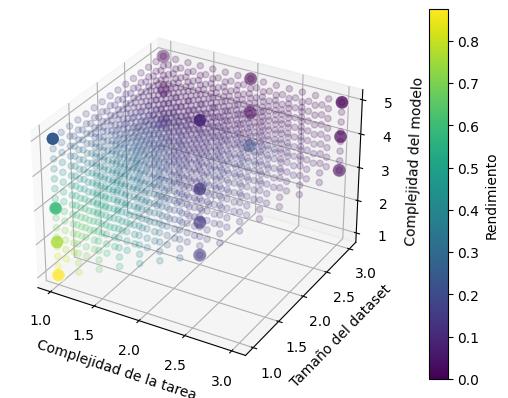
\includegraphics[width=0.75\linewidth]{Plantilla_TFG_latex//imagenes//Inf//Resultados/P3/3d.png}
    \caption{Representación del rendimiento medio reescalado de las técnicas metaheurísticas según la complejidad de la tarea, el tamaño del conjunto de datos y la complejidad del modelo.}
    \label{fig:3dP1}
\end{figure}

Visualicemos los vectores que hemos descrito como puntos en un espacio tridimensional, asignando una escala de color para medir el rendimiento. Como vemos en la figura \ref{fig:3dP1}, el tamaño del conjunto de datos parece ser el factor que más influye en el rendimiento de un modelo entrenado a través de metaheurísticas. 



Analizando dos a dos estos tres factores, a través de un mapa de calor, vemos en la figura \ref{fig:hmP1} que la complejidad del modelo también influye notablemente, siendo con la que más varía el rendimiento en esta representación.

\begin{figure}[!tbp]
    \centering
    \subfloat{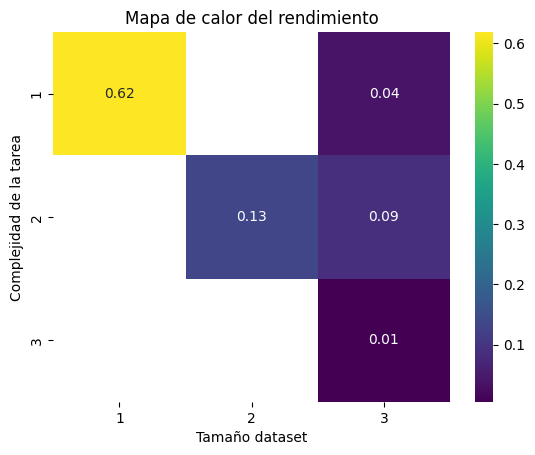
\includegraphics[width=0.5\textwidth]{Plantilla_TFG_latex//imagenes//Inf//Resultados/P3/hm1.png}} 
    \hfill
    \subfloat{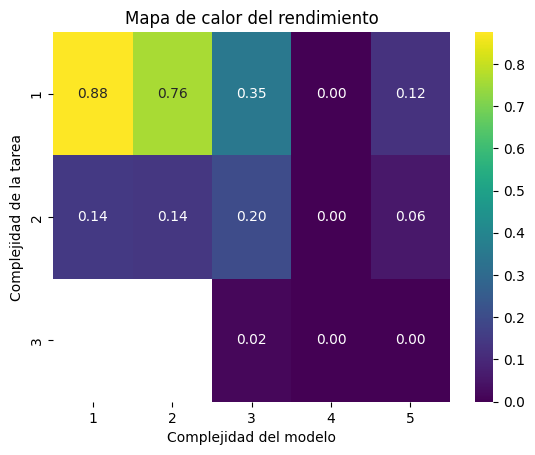
\includegraphics[width=0.5\textwidth]{Plantilla_TFG_latex//imagenes//Inf//Resultados/P3/hm2.png}} 
    \hfill
    \subfloat{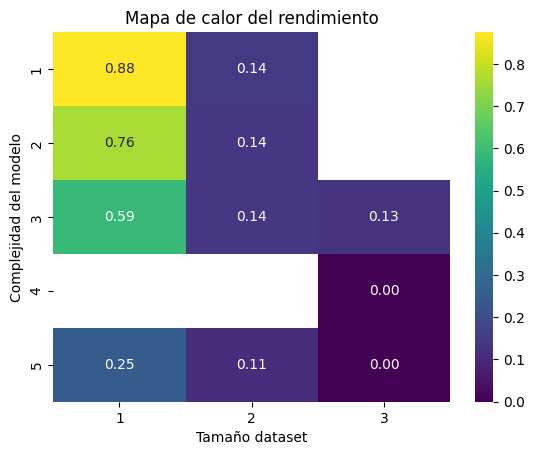
\includegraphics[width=0.5\textwidth]{Plantilla_TFG_latex//imagenes//Inf//Resultados/P3/hm3.png}} 
    \caption{Mapa de calor del rendimiento de las técnicas metaheurísticas analizando dos a dos tres factores: complejidad de la tarea, tamaño del conjunto de datos y complejidad del modelo.}
    \label{fig:hmP1}
\end{figure}


En último lugar, realizaremos un análisis de dependencias parciales para evaluar cómo cada una de estas tres variantes afecta al rendimiento, utilizando un modelo de regresión con \textit{Random Forest} \cite{randomforest}. Al observar los resultados en \ref{fig:P1rf} confirmamos que nuestras afirmaciones son correctas y podemos cuantificarlas.

Nuestros resultados muestran que el tamaño del conjunto de datos es el factor más influyente en el rendimiento de modelos entrenados con técnicas metaheurísticas, superando significativamente la influencia de la complejidad del modelo. Aunque ésta también influye en el rendimiento, lo hace en menor medida. Por otro lado, la complejidad de la tarea parece tener un impacto mínimo.

En conclusión, la cantidad de datos del conjunto es el principal factor que determina el rendimiento de la técnicas metaheurísticas, seguido por el número de parámetros del modelo, mientras que la complejidad de la tarea tiene un impacto mucho menor.

\begin{figure}
    \centering
    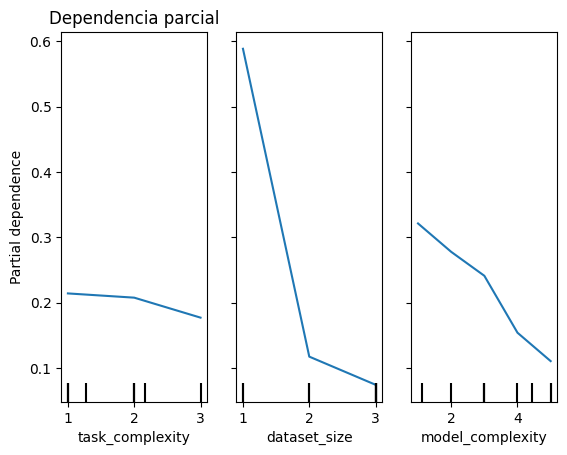
\includegraphics[width=0.75\linewidth]{Plantilla_TFG_latex//imagenes//Inf//Resultados/P3/dependencia_parcial.png}
    \caption{Análisis de dependencias parciales en base al rendimiento de los modelos entrenados con técnicas metaheurísticas según la complejidad de la tarea, el tamaño del conjunto de datos y la complejidad del modelo.}
    \label{fig:P1rf}
\end{figure}




%%%%%%%%%%%%%%%%%%%%%%%%%%%%%%%%%%%%%%%%%%%%%%%%%%%%%%%%%%%%

\subsection{Cuestión P2}

\begin{table}[H]
\centering
\begin{tabular}{|c|c|c|c|c|}
\hline
\backslashbox{Algoritmo}{Capas} & 1            & 2            & 5            & 11   \\ \hline
NAG                             & 2.5          & 2.5          & 2.6          & 3.1  \\ \hline
RMSPROP                         & 2.4 & 2.4 & 2.6 & 3.1  \\ \hline
ADAM                            & 2.4          & 2.4          & 2.9          & 3.0  \\ \hline
SHADE                           & 126          & 135          & 214          & 1265 \\ \hline
SHADE-ILS                       & 135          & 147          & 251          & 1789 \\ \hline
SHADE-GD                        & 200          & 220          & 315          & 1779 \\ \hline
SHADE-ILS-GD                    & 210          & 224          & 368          & 2171 \\ \hline
\end{tabular}
\caption{Tiempo del entrenamiento en segundos para el conjunto de datos Breast Cancer Winsconsin.}
\label{tab:bcw_time}
\end{table}


\begin{table}[H]
\centering
\begin{tabular}{|c|c|c|c|c|}
\hline
\backslashbox{Algoritmo}{Capas} & 1      & 2      & 5       & 11      \\ \hline
NAG                             & 9.47   & 10.24  & 12.58   & 15.45   \\ \hline
RMSPROP                         & 9.69   & 10.06  & 12.28   & 17.92   \\ \hline
ADAM                            & 9.88   & 10.76  & 12.67   & 17.31   \\ \hline
SHADE                           & 708.60 & 770.07 & 969.46  & 1941.44 \\ \hline
SHADE-ILS                       & 798.46 & 864.93 & 1108.06 & 2390.91 \\ \hline
SHADE-GD                        & 800.24 & 854.46 & 1096.99 & 2096.57 \\ \hline
SHADE-ILS-GD                    & 799.41 & 867.99 & 1098.78 & 2247.98 \\ \hline
\end{tabular}
\caption{Tiempo del entrenamiento en segundos para el dataset Wine Quality (Clasificación).}
\label{tab:wqc_time}
\end{table}

Ahora realizaremos un análisis de la complejidad computacional de las metaheurísticas en relación con el tiempo de entrenamiento. Vamos observar los tiempos de entrenamiento en los conjuntos de datos de BCW (\ref{tab:bcw_time}, WQC (\ref{tab:wqc_time} y F-MNIST (\ref{tab:fmnist_time}), que representan de menor a mayor la cantidad de datos utilizados. En la tabla \ref{tab:timesmaxmin}, se muestran las mayores y menores diferencias diferencias de tiempo para estos tres conjuntos, siendo la mayor del orden de 723 veces mayor. 

Se puede observar que la menor diferencia siempre se presenta en el modelo con el menor número de parámetros, a excepción del conjunto de datos WQC, donde se da en el modelo MLP de 2 capas, que tiene un número de parámetros similar al de 1 capa. Por otro lado, la mayor diferencia se registra consistentemente en el modelo con el mayor número de parámetros. Por lo tanto, podemos concluir que el número de parámetros del modelo que entrenamos afecta negativamente al tiempo consumido por las técnicas metaheurísticas en comparación con los optimizadores basados en gradiente.



\begin{table}[H]
\centering
\begin{tabular}{|c|c|c|c|}
\hline
\backslashbox{Algoritmo}{Modelo} & LeNet5  & ResNet15 & ResNet57 \\ \hline
NAG                              & 59.74   & 61.10    & 74.48    \\ \hline
RMSPROP                          & 56.92   & 63.98    & 73.48    \\ \hline
ADAM                             & 56.41   & 63.56    & 73.59    \\ \hline
SHADE                            & 6699.62 & 7233.42  & 8500.08  \\ \hline
SHADE-ILS                        & 5999.57 & 6668.34  & 10846.33 \\ \hline
SHADE-GD                         & 6466.79 & 7028.41  & 10474.43 \\ \hline
SHADE-ILS-GD                     & 6641.35 & 7238.65  & 8900.86  \\ \hline
\end{tabular}
\caption{Tiempo del entrenamiento en segundos para el conjunto de datos F-MNIST.}
\label{tab:fmnist_time}
\end{table}

% Please add the following required packages to your document preamble:
% \usepackage{multirow}
\begin{table}[]
\resizebox{\textwidth}{!}{\begin{tabular}{|cc|c|c|c|c|}
\hline
\multicolumn{2}{|c|}{\textbf{Medida}}                             & \textbf{Veces mayor} & \textbf{Capas/modelo} & \textbf{Optimizador} & \textbf{Técnica MH} \\ \hline
\multicolumn{1}{|c|}{\multirow{2}{*}{BCW}}     & Mayor diferencia & 723.67               & 11                    & ADAM                 & SHADE-ILS-GD        \\ \cline{2-6} 
\multicolumn{1}{|c|}{}                         & Menor diferencia & 50.4                 & 1                     & NAG                  & SHADE               \\ \hline
\multicolumn{1}{|c|}{\multirow{2}{*}{WQC}}     & Mayor diferencia & 154.77               & 11                    & NAG                  & SHADE-ILS           \\ \cline{2-6} 
\multicolumn{1}{|c|}{}                         & Menor diferencia & 71.57                & 2                     & ADAM                 & SHADE               \\ \hline
\multicolumn{1}{|c|}{\multirow{2}{*}{F-MNIST}} & Mayor diferencia & 147.60               & ResNet57              & RMSPROP              & SHADE-ILS           \\ \cline{2-6} 
\multicolumn{1}{|c|}{}                         & Menor diferencia & 100.42               & LeNet5               & NAG                  & SHADE-ILS           \\ \hline
\end{tabular}}
\caption{Mayores y menores diferencias de tiempo, expresada en veces mayor, de los entrenamientos en los conjuntos de datos de BCW, WQC y F-MNIST, entre las técnicas metaheurísticas y optimizadores basados en gradiente descendente.}
\label{tab:timesmaxmin}
\end{table}

Además, en esa misma tabla podemos apreciar que, a medida que aumenta el tamaño del conjunto de datos, tanto la menor como la mayor diferencia van reduciendo su separación. Esto sugiere que, si continuáramos aumentando el número de datos, estas diferencias se acercarían más entre sí. Aunque no podemos afirmar que converjan a una cierta proporción, podríamos suponer que ambas quedarían dentro de un intervalo que podríamos calcular teóricamente.


Vamos a analizar la complejidad computacional observando primero de dónde surgen estas diferencias de tiempo. Para el manejo de las metaheurísticas, hemos implementado una función de error propia, así que compararemos el tiempo base que requiere. Es importante recalcar que dicha función está basada en la de PyTorch y utiliza la librería CUDA para acelerar los cálculos.

Medimos el tiempo necesario en realizar una época con el optimizador Adam, con los modelos LeNet5 y ResNet57 en F-MNIST; y cuánto tarda en ejecutar la la función de error implementada. Es relevante tener en cuenta que, con la implementación que hemos realizado de las metaheurísticas, el error de validación y el valor de \textit{accuracy} se calculan a posteriori y, por tanto, no se incluyen en la medición del tiempo de las metaheurísticas. Observamos los resultados, ejecutados en F-MNIST, en la tabla \ref{tab:base_time}.

\begin{table}[]
\centering
\begin{tabular}{c|c|c|c|c|}
\cline{2-5}
                                                                     & LeNet5 & ResNet57 & MLP 1 capa & MLP 11 capas \\ \hline
\multicolumn{1}{|c|}{Adam}                                           & 3.9    & 4.0      & 0.49       & 0.76         \\ \hline
\multicolumn{1}{|c|}{Función1}              & 1.54   & 1.62     & 0.16       & 0.31         \\ \hline
\multicolumn{1}{|c|}{Función2} & 4.47   & 4.34     & 0.24       & 0.44         \\ \hline
\end{tabular}
\caption{Comparación de los tiempos de ejecución para una época de Adam, la función de error implementada sobre el conjunto de entrenamiento (Función1), y la función de error implementada para el conjunto de entrenamiento, de validación y el cálculo de \textit{accuracy} (Función2), para los diferentes modelos indicados y en F-MNIST.}
\label{tab:base_time}
\end{table}


%%%
La diferencia de tiempo entre el gradiente descendente y la función de error sobre el conjunto de entrenamiento es evidente, ya que se están realizando muchas menos operaciones y procesando menos datos. La discrepancia con respecto al tiempo total de la función de error propia se debe a que, al trabajar con metaheurísticas, es necesario obtener explícitamente las predicciones del modelo y las etiquetas reales de los datos, lo que implica realizar un pase hacia adelante adicional en el modelo, lo que consume ese tiempo adicional. En el caso de la evaluación con Adam, no es necesario realizar este pase, ya que, al utilizar \textit{backpropagation} y la diferenciación automática, podemos aprovechar y almacenar los datos intermedios al calcular el error para reutilizarlos posteriormente.

Continuaremos con el análisis utilizando como referencia la función de error sobre el conjunto de entrenamiento únicamente, ya que los tiempos obtenidos de las ejecuciones de los algoritmos no tienen en cuenta el conjunto de validación ni es cálculo de \textit{accuracy}. Una pregunta pertinente en este punto es: sabiendo el tiempo que tarda en ejecutarse la función de error y cuántas veces se ejecuta a lo largo del entrenamiento con una técnica metaheurística, ¿cuánto debería tardar teóricamente en ejecutarse nuestro algoritmo? Teniendo en cuenta que realizamos aproximadamente 4200 evaluaciones de la función de coste, podemos realizar un sencillo cálculo que nos da como resultado 6481.22 segundos en el caso de LeNet5 y 6812.37 segundos en el caso de ResNet57. Aquí comienzan a notarse las diferencias debido al distinto número de parámetros. En el primer caso, el tiempo se ajusta bastante a la realidad; sin embargo, en el segundo, la discrepancia con respecto a los valores de la tabla \ref{tab:fmnist_time} es bastante significativa.

Vamos a analizar de dónde pueden surgir estas diferencias en los tiempos. Aproximaremos los tiempos a partir del algoritmo SHADE. Es importante tener en cuenta cuáles son las operaciones que más tiempo consumen por generación; en este caso, está claro que son el cruce, la mutación y la evaluación del error, mientras que despreciamos el resto de operaciones. Por lo tanto, los 218.4 segundos de diferencia corresponden a las operaciones de cruce y mutación.

Vamos a suponer que la operación de cruce y la de mutación tardan lo mismo en ejecutarse, ya que simplificará el análisis y llegaremos a los mismos resultados. En dicho algoritmo, por cada elemento de la población y en cada generación, se realiza un cruce, una mutación y una evaluación de la función de error del nuevo individuo generado. Dado que realizamos 4200 evaluaciones de la función objetivo y tenemos 10 individuos, tendremos 420 generaciones, lo que equivale a un total de 840 operaciones entre cruces y mutaciones. Por lo tanto, concluimos que cada operación requiere aproximadamente 0.26 segundos para su ejecución.

Dichas funciones no hacen uso de la librería CUDA, por lo que presumiblemente aumentarán el tiempo empleado en mayor medida cuando aumente el número de parámetros del modelo, es decir, el número de datos con los que deben operar. Es importante mencionar que aquí encontramos una limitación en la estructura de datos, ya que en la implementación de las metaheurísticas estamos abandonando la estructura por capas de las redes neuronales y utilizando \textit{arrays}. Esto significa que no usar estas librerías es más bien una incapacidad y no una elección. Suponiendo, por lo tanto, que los 1688.11 segundos de diferencia entre nuestro cálculo teórico y el tiempo real consumido por SHADE al entrenar el modelo ResNet57 provienen de estas operaciones, eso equivaldría a que cada operación tarda aproximadamente 2 segundos, lo que representa unas 8 veces más que en el caso anterior.

Haciendo el mismo análisis para WQC, obtenemos que las funciones de cruce y mutación consumen 0.04 segundos en el caso del MLP de 1 capa y 2.31 segundos en el caso de 11 capas. Sabiendo que la función de error depende del número de datos y del número de parámetros del modelo, mientras que las funciones de cruce y mutación dependen únicamente del número de parámetros del modelo, con los datos obtenidos podemos aproximar el orden de complejidad del algoritmo SHADE.

El tiempo total consumido será de $4200 \cdot func_{error} + 840 \cdot cruce\_mut$, por lo que ya podemos calcular su complejidad algoritmíca enbase al tiempo. Primero averiguamos el orden de complejidad de las funciones de cruce y mutación, tomando los pares $(dimension\_del\_modelo, tiempo\_de\_ejecucion)$. Suponemos una complejidad $T(n)=k \cdot n^a$ y transformamos los valores a escala logarítmica.

\begin{align*}
log(d1)&=log(1306)\approx3.116\\
log(t1)&=log(0.04)\approx -1.398\\
log(d2)&=log(62,158)\approx4.793\\
log(t2)&=log(0.26)\approx-0.585\\
log(d3)&=log(1,346,826)\approx6.129\\
log(t3)&=log(2)\approx0.301\\
log(d4)&=log(1,403,354)\approx6.148\\
log(t4)&=log(3.21)\approx1.165.
\end{align*}


Tenemos que $log(T)=log(k) + a \cdot log(d)$. A través de una regresión lineal utilizando los datos anteriores obtenemos que $a = 0.549$ y $log(k)=-7.236$, es decir $k=e^{-7.236}$. Por tanto estas funciones tienen una complejidad de $T(p) = e^{-7.236}\cdot p^{0.549}$, donde $p$ representa el número de parámetros del modelo.

Realizamos el mismo proceso para la función de error, que depende del tamaño del conjunto de datos y el número de parámetros del modelo. Entonces, suponemos $T(p,d)=k \cdot p^a \cdot d^b$, y después de la regresión obtenemos $T(p,d)=e^{-7.25} \cdot p^{0.42} \cdot d^{0.12}$, donde $p$ es el número de parámetros del modelo y $d$ el tamaño del conjunto de datos. Podemos establecer entonces que el orden de complejidad del algoritmo SHADE es


\begin{align*}
T(p,d)&= N_{eval} \cdot e^{-7.25} \cdot p^{0.42} \cdot d^{0.12} + \frac{N_{eval}}{Tam_{pob}} \cdot e^{-7.236}\cdot p^{0.549} \\
          &= O( p^{0.42} \cdot d^{0.12}) + O(p^{0.549}).
\end{align*}

En la práctica, el segundo término domina al tener un mayor exponente, especialmente considerando que en los entrenamientos de modelos de aprendizaje profundo actuales el número de parámetros suele ser mucho mayor que la cantidad de datos. Por lo tanto, de manera general, se tiene $T(p)=O(p^{0.549})$. Respondiendo finalmente a la cuestión, afirmamos que tanto el número de datos como el número de parámetros del modelo afectan, y acabamos de ver de qué manera, al tiempo consumido en el entrenamiento a través de metaheurísticas; además, el número de parámetros afecta en mayor medida. Otra conclusión interesante es que los factores de cruce y mutación son mucho más determinantes que la evaluación del error, aunque esto esté marcado por los motivos que hemos mencionado antes, como la imposibilidad de usar CUDA.


%%%%%%%%%%%%%%%%%%%%%%%%%%%%%%%%%%%%%%%%%%%%%%



\subsection{Cuestión P3}

Para observar si existe alguna diferencia en el rendimiento de las técnicas metaheurísticas al enfrentarse a la tarea de regresión o clasificación, vamos a comparar los resultados de los cuatro conjuntos de datos tabulares. Contamos con dos tareas de clasificación y dos tareas de regresión, con dificultades de la tarea y tamaño del conjunto de datos similares dos a dos, como se observa en la tabla \ref{tab:expP3}.

\begin{table}[]
\centering
\resizebox{\textwidth}{!}{\begin{tabular}{|c|c|c|c|}
\hline
\textbf{Conjunto de datos} & \textbf{Tarea} & \textbf{Complejidad} & \textbf{Cantidad de datos} \\ \hline
\textbf{BCW}               & Clasificación  & Fácil                & Poca                       \\ \hline
\textbf{BHP}               & Regresión      & Fácil                & Poca                       \\ \hline
\textbf{WQC}               & Clasificación  & Media                & Intermedia                 \\ \hline
\textbf{WQR}               & Regresión      & Media                & Intermedia                 \\ \hline
\end{tabular}}
\caption{Tareas a comparar para la cuestión P3.}
\label{tab:expP3}
\end{table}

% Please add the following required packages to your document preamble:
% \usepackage{multirow}
\begin{table}[]
\resizebox{\textwidth}{!}{\begin{tabular}{|c|ccc|ccc|ccc|ccc|}
\hline
\multirow{2}{*}{\textbf{Capas}} & \multicolumn{3}{c|}{\textbf{SHADE}}                          & \multicolumn{3}{c|}{\textbf{SHADE-ILS}}                                                 & \multicolumn{3}{c|}{\textbf{SHADE-GD}}                                                  & \multicolumn{3}{c|}{\textbf{SHADE-ILS-GD}}                   \\ \cline{2-13} 
                                & \multicolumn{1}{c|}{E}    & \multicolumn{1}{c|}{T}    & M    & \multicolumn{1}{c|}{E}             & \multicolumn{1}{c|}{T}             & M             & \multicolumn{1}{c|}{E}             & \multicolumn{1}{c|}{T}             & M             & \multicolumn{1}{c|}{E}    & \multicolumn{1}{c|}{T}    & M    \\ \hline
\textbf{1}                      & \multicolumn{1}{c|}{0.10} & \multicolumn{1}{c|}{0.18} & 0.93 & \multicolumn{1}{c|}{\textbf{0.07}} & \multicolumn{1}{c|}{\textbf{0.14}} & \textbf{0.97} & \multicolumn{1}{c|}{0.10}          & \multicolumn{1}{c|}{0.18}          & 0.91          & \multicolumn{1}{c|}{0.06} & \multicolumn{1}{c|}{0.15} & 0.94 \\ \hline
\textbf{2}                      & \multicolumn{1}{c|}{0.21} & \multicolumn{1}{c|}{0.49} & 0.72 & \multicolumn{1}{c|}{0.06}          & \multicolumn{1}{c|}{0.35}          & 0.93          & \multicolumn{1}{c|}{\textbf{0.11}} & \multicolumn{1}{c|}{\textbf{0.22}} & \textbf{0.95} & \multicolumn{1}{c|}{0.06} & \multicolumn{1}{c|}{0.35} & 0.93 \\ \hline
\textbf{5}                      & \multicolumn{1}{c|}{0.63} & \multicolumn{1}{c|}{0.64} & 0.82 & \multicolumn{1}{c|}{\textbf{0.05}} & \multicolumn{1}{c|}{\textbf{0.47}} & \textbf{0.89} & \multicolumn{1}{c|}{0.10}          & \multicolumn{1}{c|}{0.45}          & 0.87          & \multicolumn{1}{c|}{0.03} & \multicolumn{1}{c|}{0.61} & 0.6  \\ \hline
\textbf{11}                     & \multicolumn{1}{c|}{0.70} & \multicolumn{1}{c|}{0.67} & 0.5  & \multicolumn{1}{c|}{\textbf{0.09}} & \multicolumn{1}{c|}{\textbf{0.49}} & \textbf{0.90} & \multicolumn{1}{c|}{0.27}          & \multicolumn{1}{c|}{0.65}          & 0.60          & \multicolumn{1}{c|}{0.11} & \multicolumn{1}{c|}{0.70} & 0.50 \\ \hline
\end{tabular}}
\caption{Entrenamiento de las técnicas metaheurísticas en el conjunto de datos BCW. E: Entrenamiento, T: Test, A: \textit{Accuracy}.}
\label{tab:P3bcw}
\end{table}

% Please add the following required packages to your document preamble:
% \usepackage{multirow}
\begin{table}[]
\resizebox{\textwidth}{!}{\begin{tabular}{|c|ccc|ccc|ccc|ccc|}
\hline
\multirow{2}{*}{\textbf{Capas}} & \multicolumn{3}{c|}{\textbf{SHADE}}                                                     & \multicolumn{3}{c|}{\textbf{SHADE-ILS}}                      & \multicolumn{3}{c|}{\textbf{SHADE-GD}}                       & \multicolumn{3}{c|}{\textbf{SHADE-ILS-GD}}                                              \\ \cline{2-13} 
                                & \multicolumn{1}{c|}{E}             & \multicolumn{1}{c|}{T}             & A             & \multicolumn{1}{c|}{E}    & \multicolumn{1}{c|}{T}    & A    & \multicolumn{1}{c|}{E}    & \multicolumn{1}{c|}{T}    & A    & \multicolumn{1}{c|}{E}             & \multicolumn{1}{c|}{T}             & A             \\ \hline
\textbf{1}                      & \multicolumn{1}{c|}{\textbf{2.08}} & \multicolumn{1}{c|}{\textbf{2.16}} & \textbf{0.30} & \multicolumn{1}{c|}{1.04} & \multicolumn{1}{c|}{1.05} & 0.22 & \multicolumn{1}{c|}{0.98} & \multicolumn{1}{c|}{1.11} & 0.20 & \multicolumn{1}{c|}{1.03}          & \multicolumn{1}{c|}{1.09}          & 0.20          \\ \hline
\textbf{2}                      & \multicolumn{1}{c|}{2.12}          & \multicolumn{1}{c|}{2.55}          & 0.21          & \multicolumn{1}{c|}{1.05} & \multicolumn{1}{c|}{1.11} & 0.20 & \multicolumn{1}{c|}{0.91} & \multicolumn{1}{c|}{1.09} & 0.20 & \multicolumn{1}{c|}{\textbf{0.99}} & \multicolumn{1}{c|}{\textbf{10.4}} & \textbf{0.29} \\ \hline
\textbf{5}                      & \multicolumn{1}{c|}{2.58}          & \multicolumn{1}{c|}{2.30}          & 0.15          & \multicolumn{1}{c|}{0.93} & \multicolumn{1}{c|}{1.07} & 0.23 & \multicolumn{1}{c|}{0.99} & \multicolumn{1}{c|}{1.00} & 0.25 & \multicolumn{1}{c|}{\textbf{0.96}} & \multicolumn{1}{c|}{\textbf{1.05}} & \textbf{0.27} \\ \hline
\textbf{11}                     & \multicolumn{1}{c|}{2.51}          & \multicolumn{1}{c|}{2.30}          & 0.20          & \multicolumn{1}{c|}{0.96} & \multicolumn{1}{c|}{1.14} & 0.20 & \multicolumn{1}{c|}{1.01} & \multicolumn{1}{c|}{1.24} & 0.20 & \multicolumn{1}{c|}{0.48}          & \multicolumn{1}{c|}{1.37}          & 0.20          \\ \hline
\end{tabular}}
\caption{Entrenamiento de las técnicas metaheurísticas en el conjunto de datos WQC. E: Entrenamiento, T: Test, A: \textit{Accuracy}.}
\label{tab:P3wqc}
\end{table}

Podemos ver los resultados del entrenamiento en las tablas \ref{tab:P3bcw} y \ref{tab:P3wqc}. Como se observa, las tareas con menor cantidad de datos y mayor facilidad logran un mejor rendimiento. Es importante prepararnos adecuadamente para realizar la comparación, ya que las funciones de pérdida y las métricas son diferentes en clasificación y regresión. Además, en las dos tareas de clasificación, el número de clases varía, lo que también afecta el rendimiento del clasificador aleatorio que utilizaremos como referencia. Por lo tanto, aplicaremos el mismo proceso que realizamos en el análisis de la cuestión \textit{P1} y pondremos dichas métricas en una escala de [0,1], donde 0 representa el rendimiento del clasificador aleatorio correspondiente.



Compararemos las métricas \textit{accuracy} (con la correspondiente transformación) y R$^2$, ya que ofrecen una interpretación similar. La primera indica el rendimiento de nuestro modelo en función del rendimiento del clasificador aleatorio, mientras que la segunda se refiere a cuán bien se predicen los datos usando la media. Esto también soluciona el problema de las distintas escalas en las tareas de regresión. Ahora que contamos con un criterio objetivo para comparar, evaluaremos el rendimiento medio de cada técnica metaheurística agrupando en función de la cantidad de datos y la complejidad del modelo, que son los dos factores que más influyen en el rendimiento, tal como hemos observado. Compararemos respecto al rendimiento obtenido por las técnicas de gradiente descendente, de manera que no nos influya la complejidad de la tarea en la comparación. Como hemos mencionado, este es el factor que menos influye de los tres, y podemos suponer que si el rendimiento disminuye con unas técnicas, también lo hará con otras.

\begin{figure}[!tbp]
    \centering
    \subfloat{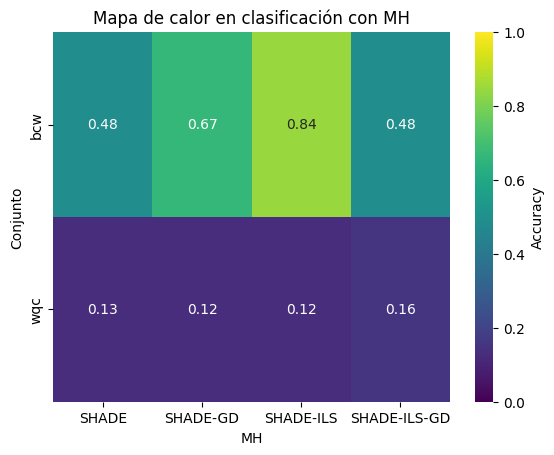
\includegraphics[width=0.5\textwidth]{Plantilla_TFG_latex//imagenes//Inf//Resultados/P2/data_clas_mh.png}} 
    \hfill
    \subfloat{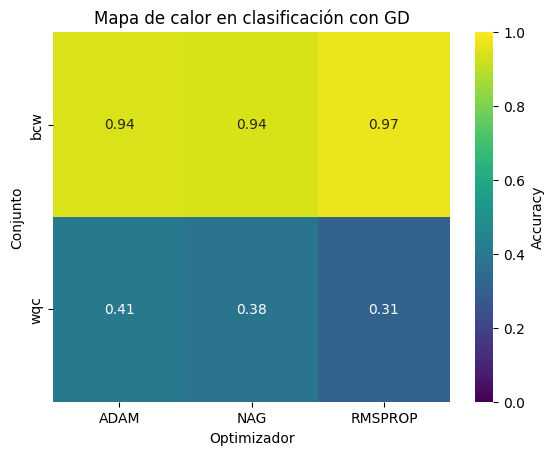
\includegraphics[width=0.5\textwidth]{Plantilla_TFG_latex//imagenes//Inf//Resultados/P2/data_clas_gd.png}} 
    \hfill
    \subfloat{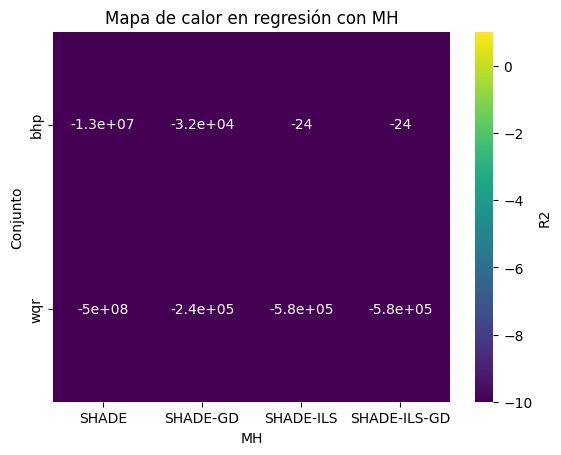
\includegraphics[width=0.5\textwidth]{Plantilla_TFG_latex//imagenes//Inf//Resultados/P2/data_reg_mh.png}} 
    \hfill
    \subfloat{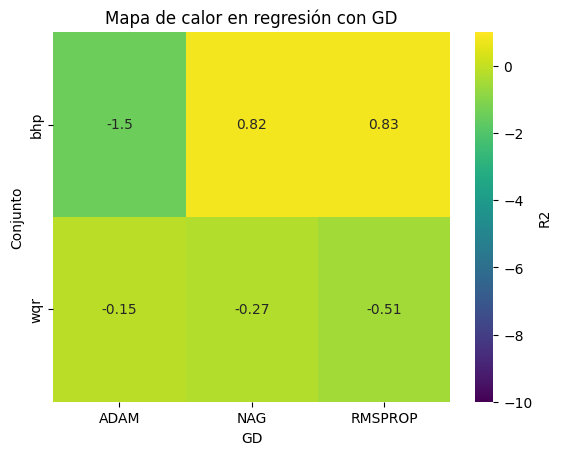
\includegraphics[width=0.5\textwidth]{Plantilla_TFG_latex//imagenes//Inf//Resultados/P2/data_reg_gd.png}} 
    \caption{Mapa de calor del rendimiento de las técnicas metaheurísticas para los datasets correspondientes, realizando una media de los valores entre las distintas capas.}
    \label{fig:P3hmdata}
\end{figure}

En la figura\ref{fig:P3hmdata} obervamos los resultados medios en base a los conjuntos de datos, mientras que en \ref{fig:P3hmlayer} los resultados están agrupados por capas. A simple vista, podríamos concluir que los resultados en regresión son peores que los de clasificación en comparación con el gradiente descendente, y que por tanto sí que existe una diferencia entre estas dos tareas en cuanto al rendimiento de las técnicas metaheurísticas. Sin embargo, para afirmar esto con certeza, llevaremos a cabo la prueba de los rangos con signo de Wilcoxon, que es una alternativa al test t-Student cuando los datos no siguen una distribución normal y las dos muestras están relacionadas, como es nuestro caso. Hemos decidido aplicar la prueba de Wilcoxon tras verificar, mediante el test de Shapiro-Wilk, que los datos no siguen una distribución normal.


\begin{figure}[!tbp]
    \centering
    \subfloat{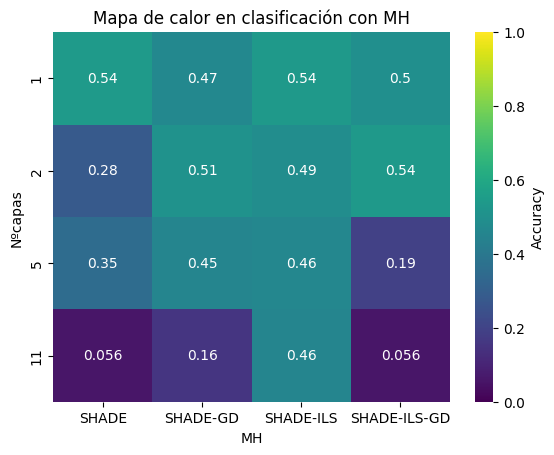
\includegraphics[width=0.5\textwidth]{Plantilla_TFG_latex//imagenes//Inf//Resultados/P2/layer_clas_mh.png}} 
    \hfill
    \subfloat{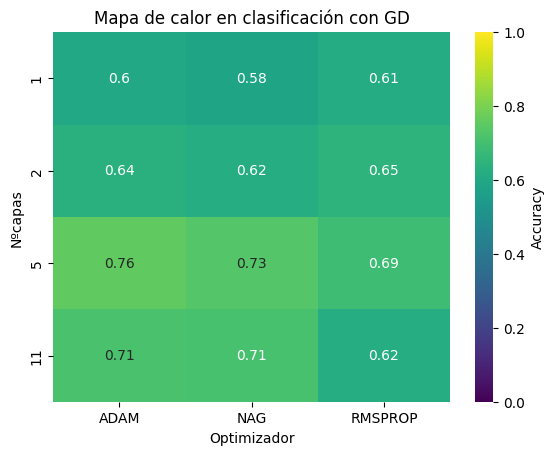
\includegraphics[width=0.5\textwidth]{Plantilla_TFG_latex//imagenes//Inf//Resultados/P2/layer_clas_gd.png}} 
    \hfill
    \subfloat{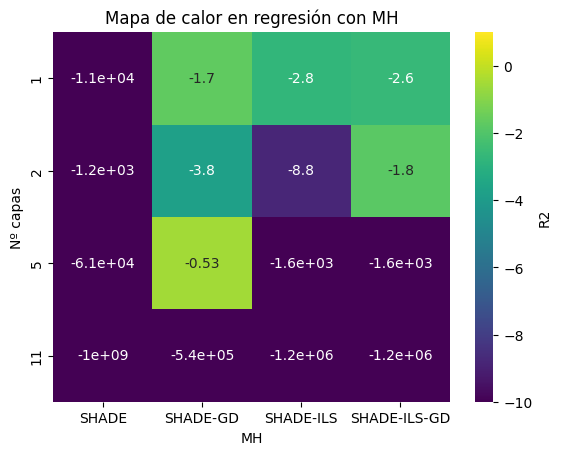
\includegraphics[width=0.5\textwidth]{Plantilla_TFG_latex//imagenes//Inf//Resultados/P2/layer_reg_mh.png}} 
    \hfill
    \subfloat{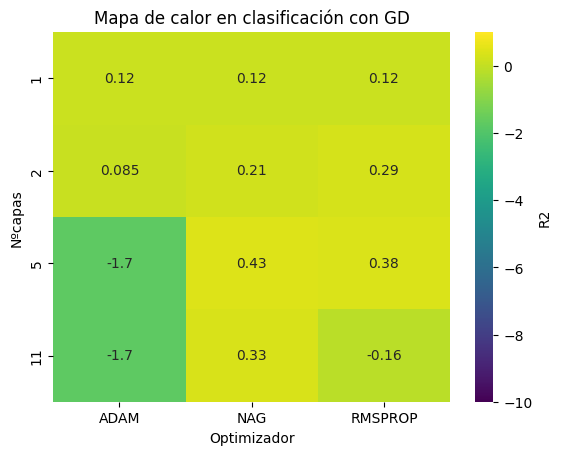
\includegraphics[width=0.5\textwidth]{Plantilla_TFG_latex//imagenes//Inf//Resultados/P2/layer_reg_gd.png}} 
    \caption{Mapa de calor del rendimiento de las técnicas metaheurísticas para los distintos números de capas de los modelos MLP, realizando una media de los valores entre los conjuntos de datos correspondientes.}
    \label{fig:P3hmlayer}
\end{figure}

Compararemos dos distribuciones: una será la diferencia de rendimiento de las técnicas metaheurísticas con respecto al gradiente descendente en tareas de regresión, y la otra será equivalente, pero en problemas de clasificación. Si encontramos una diferencia entre ambas distribuciones, confirmaremos que existe una variación en el rendimiento de las técnicas metaheurísticas en tareas de clasificación y regresión.


Se podría alegar que existe un sesgo en el rendimiento de las métricas, ya que R$^2$ no tiene límite inferior; un modelo muy malo podría hacer que este valor decrezca infinitamente. Esto contrasta con la métrica que usamos en clasificación, que sí tiene un límite y se alcanza en varios casos (véase un valor de 0.5 en BCW y 0.2\footnote{Teóricamente sería un 10\% el valor que obtendría en este caso el clasificador aleatorio, pero hay un sutil detalle que cambia esto y que se comenta en la sección anterior} en WQC). Por tanto vamos a ejecutar la prueba sobre los valores de las métricas, el error de entrenamiento y el error de generalización para evitar este posible sesgo.

La función de entropía cruzada tiene un valor teórico máximo, pero los modelos entrenados no se acercan a él. Este valor se alcanzaría cuando predecimos con un 0\% de probabilidad la clase correcta, lo que daría lugar a un error con valor de $-log(0) \approx + \infty$. Sin embargo, en las implementaciones de las librerías de aprendizaje automático se utiliza un valor muy pequeño para evitar evaluar la función en un punto en el que no esté definida. Suponiendo que este valor sea $10^{-8}$, que es muy común en la literatura para prevenir divisiones por cero, el valor máximo teórico de la función de entropía cruzada sería aproximadamente 18.42. Esto es muy lejano a los errores cometidos por los modelos entrenados, que son todos menores a 4. Por tanto concluimos los valores del error de generalización no están limitados y, en consecuencia, no existe dicho sesgo.


Nuestra hipótesis nula será que no existe diferencia en el rendimiento de los modelos entrenados con técnicas metaheurísticas en comparación con su versión entrenada mediante gradiente descendente, tanto para tareas de clasificación como de regresión. La hipótesis alternativa, por otro lado, postula que sí existe una diferencia en el rendimiento. En total, formularemos tres hipótesis, correspondientes a los tres medidores mencionados anteriormente. Estableceremos un nivel de significación de 0.05, que es un valor comúnmente aceptado en estudios estadísticos.

Los resultados del test se muestran en la tabla \ref{tab:test}. Dado que estos resultados se encuentran por debajo del nivel de significación establecido, podemos afirmar con firmeza que existe una diferencia en el rendimiento de las técnicas metaheurísticas en tareas de clasificación y regresión.

\begin{table}[]
\centering
\begin{tabular}{|c|c|c|}
\hline
\textbf{Medida}      & \textbf{Estadístico} & \textbf{P-valor} \\ \hline
Error entrenamiento  & 80.0                 & 0.045            \\ \hline
Error generalización & 14.0                 & 0.00001          \\ \hline
Métrica              & 25.0                 & 0.0001           \\ \hline
\end{tabular}
\caption{Valores del test de Wilcoxon para las hipótesis propuestas.}
\label{tab:test}
\end{table}




% Please add the following required packages to your document preamble:
% \usepackage{multirow}
\begin{table}[]
\resizebox{\textwidth}{!}{\begin{tabular}{|cc|c|c|c|c|}
\hline
\multicolumn{2}{|c|}{\textbf{Medida}}                             & \textbf{Veces mayor} & \textbf{Capas/modelo} & \textbf{Optimizador} & \textbf{Técnica MH} \\ \hline
\multicolumn{1}{|c|}{\multirow{2}{*}{BCW}}     & Mayor diferencia & 723.67               & 11                    & ADAM                 & SHADE-ILS-GD        \\ \cline{2-6} 
\multicolumn{1}{|c|}{}                         & Menor diferencia & 50.4                 & 1                     & NAG                  & SHADE               \\ \hline
\multicolumn{1}{|c|}{\multirow{2}{*}{WQC}}     & Mayor diferencia & 154.77               & 11                    & NAG                  & SHADE-ILS           \\ \cline{2-6} 
\multicolumn{1}{|c|}{}                         & Menor diferencia & 71.57                & 2                     & ADAM                 & SHADE               \\ \hline
\multicolumn{1}{|c|}{\multirow{2}{*}{F-MNIST}} & Mayor diferencia & 147.60               & ResNet57              & RMSPROP              & SHADE-ILS           \\ \cline{2-6} 
\multicolumn{1}{|c|}{}                         & Menor diferencia & 100.42               & LeNet5               & NAG                  & SHADE-ILS           \\ \hline
\end{tabular}}
\caption{Mayores y menores diferencias de tiempo, expresada en veces mayor, de los entrenamientos en los conjuntos de datos de BCW, WQC y F-MNIST, entre las técnicas metaheurísticas y optimizadores basados en gradiente descendente.}
\label{tab:timesmaxmin}
\end{table}


%%%%%%%%%%%%%%%%%%%%%%%%%%%%%


\subsection{Cuestión P4}

% Please add the following required packages to your document preamble:
% \usepackage{multirow}
\begin{table}[]
\centering
\resizebox{\textwidth}{!}{\begin{tabular}{|c|c|ccc|ccc|}
\hline
\multirow{2}{*}{\textbf{Dataset}} & \multirow{2}{*}{\textbf{Capas}} & \multicolumn{3}{c|}{\textbf{SHADE}}                                                             & \multicolumn{3}{c|}{\textbf{SHADE-GD}}                                                                       \\ \cline{3-8} 
                                  &                                 & \multicolumn{1}{c|}{E}             & \multicolumn{1}{c|}{T}             & M                     & \multicolumn{1}{c|}{E}               & \multicolumn{1}{c|}{T}               & M                              \\ \hline
\multirow{4}{*}{BCW}              & 1                               & \multicolumn{1}{c|}{\textbf{0.11}} & \multicolumn{1}{c|}{\textbf{0.18}} & \textbf{0.93}         & \multicolumn{1}{c|}{0.10}            & \multicolumn{1}{c|}{0.18}            & 0.91                           \\ \cline{2-8} 
                                  & 2                               & \multicolumn{1}{c|}{0.21}          & \multicolumn{1}{c|}{0.49}          & 0.72                  & \multicolumn{1}{c|}{\textbf{0.11}}   & \multicolumn{1}{c|}{\textbf{0.22}}   & \textbf{0.95}                  \\ \cline{2-8} 
                                  & 5                               & \multicolumn{1}{c|}{0.63}          & \multicolumn{1}{c|}{0.64}          & 0.82                  & \multicolumn{1}{c|}{\textbf{0.10}}   & \multicolumn{1}{c|}{\textbf{0.45}}   & \textbf{0.87}                  \\ \cline{2-8} 
                                  & 11                              & \multicolumn{1}{c|}{0.70}          & \multicolumn{1}{c|}{0.69}          & 0.50                  & \multicolumn{1}{c|}{\textbf{0.27}}   & \multicolumn{1}{c|}{\textbf{0.65}}   & \textbf{0.60}                  \\ \hline
\multirow{4}{*}{WQC}              & 1                               & \multicolumn{1}{c|}{\textbf{2.08}} & \multicolumn{1}{c|}{\textbf{2.16}} & \textbf{0.30}         & \multicolumn{1}{c|}{0.98}            & \multicolumn{1}{c|}{1.11}            & 0.20                           \\ \cline{2-8} 
                                  & 2                               & \multicolumn{1}{c|}{2.12}          & \multicolumn{1}{c|}{2.55}          & 0.21                  & \multicolumn{1}{c|}{\textbf{0.91}}   & \multicolumn{1}{c|}{\textbf{1.09}}   & \textbf{0.20}                  \\ \cline{2-8} 
                                  & 5                               & \multicolumn{1}{c|}{2.58}          & \multicolumn{1}{c|}{2.30}          & 0.15                  & \multicolumn{1}{c|}{\textbf{0.99}}   & \multicolumn{1}{c|}{\textbf{1.00}}   & \textbf{0.25}                  \\ \cline{2-8} 
                                  & 11                              & \multicolumn{1}{c|}{2.51}          & \multicolumn{1}{c|}{2.30}          & 0.20                  & \multicolumn{1}{c|}{\textbf{1.01}}   & \multicolumn{1}{c|}{\textbf{1.24}}   & \textbf{0.20}                  \\ \hline
\multirow{4}{*}{BHP}              & 1                               & \multicolumn{1}{c|}{430.90}        & \multicolumn{1}{c|}{452.36}        & $-1.92 \times 10^{4}$ & \multicolumn{1}{c|}{\textbf{13.97}}  & \multicolumn{1}{c|}{\textbf{33.09}}  & \textbf{0.65}                  \\ \cline{2-8} 
                                  & 2                               & \multicolumn{1}{c|}{430.97}        & \multicolumn{1}{c|}{428.22}        & $-9.60 \times 10^{2}$ & \multicolumn{1}{c|}{\textbf{384.43}} & \multicolumn{1}{c|}{\textbf{128.80}} & \textbf{-4.6}                  \\ \cline{2-8} 
                                  & 5                               & \multicolumn{1}{c|}{429.71}        & \multicolumn{1}{c|}{435.00}        & $-7.32 \times 10^{3}$ & \multicolumn{1}{c|}{\textbf{396.34}} & \multicolumn{1}{c|}{\textbf{324.05}} & \textbf{-0.93}                 \\ \cline{2-8} 
                                  & 11                              & \multicolumn{1}{c|}{469.78}        & \multicolumn{1}{c|}{454.78}        & $-5.38 \times 10^{6}$ & \multicolumn{1}{c|}{\textbf{463.33}} & \multicolumn{1}{c|}{\textbf{453.89}} & \textbf{$-1.29 \times 10^{5}$} \\ \hline
\multirow{4}{*}{WQR}              & 1                               & \multicolumn{1}{c|}{35.40}         & \multicolumn{1}{c|}{32.56}         & $-2.65 \times 10^{3}$ & \multicolumn{1}{c|}{\textbf{5.14}}   & \multicolumn{1}{c|}{\textbf{0.45}}   & \textbf{-4.02}                 \\ \cline{2-8} 
                                  & 2                               & \multicolumn{1}{c|}{34.56}         & \multicolumn{1}{c|}{31.16}         & $-1.38 \times 10^{3}$ & \multicolumn{1}{c|}{\textbf{0.40}}   & \multicolumn{1}{c|}{\textbf{0.53}}   & \textbf{-2.94}                 \\ \cline{2-8} 
                                  & 5                               & \multicolumn{1}{c|}{34.75}         & \multicolumn{1}{c|}{32.20}         & $-1.14 \times 10^{5}$ & \multicolumn{1}{c|}{\textbf{6.07}}   & \multicolumn{1}{c|}{\textbf{0.87}}   & \textbf{-0.13}                 \\ \cline{2-8} 
                                  & 11                              & \multicolumn{1}{c|}{35.30}         & \multicolumn{1}{c|}{32.60}         & $-2.01 \times 10^{8}$ & \multicolumn{1}{c|}{\textbf{35.93}}  & \multicolumn{1}{c|}{\textbf{35.46}}  & \textbf{$-9.43 \times 10^{5}$} \\ \hline
\end{tabular}}
\caption{Comparación de los resultados del entrenamiento en las técnicas SHADE y SHADE-GD para los conjuntos de datos tabulares. E: Entrenamiento, T:Test, M: Métrica.}
\label{tab:shadevsshadegd}
\end{table}


% Please add the following required packages to your document preamble:
% \usepackage{multirow}
\begin{table}[]
\centering
\begin{tabular}{|c|c|ccc|ccc|}
\hline
\multirow{2}{*}{\textbf{Dataset}} & \multirow{2}{*}{\textbf{Modelo}} & \multicolumn{3}{c|}{\textbf{SHADE}}                                                     & \multicolumn{3}{c|}{\textbf{SHADE-GD}}                                                   \\ \cline{3-8} 
                                  &                                 & \multicolumn{1}{c|}{E}             & \multicolumn{1}{c|}{T}             & M             & \multicolumn{1}{c|}{E}             & \multicolumn{1}{c|}{T}             & M              \\ \hline
\multirow{3}{*}{MNIST}            & LeNet5                          & \multicolumn{1}{c|}{2.42}          & \multicolumn{1}{c|}{2.27}          & 0.17          & \multicolumn{1}{c|}{\textbf{0.10}} & \multicolumn{1}{c|}{\textbf{1.92}} & \textbf{0.529} \\ \cline{2-8} 
                                  & ResNet15                        & \multicolumn{1}{c|}{2.81}          & \multicolumn{1}{c|}{2.30}          & 0.10          & \multicolumn{1}{c|}{0.40}          & \multicolumn{1}{c|}{2.30}          & 0.10           \\ \cline{2-8} 
                                  & ResNet57                        & \multicolumn{1}{c|}{3.63}          & \multicolumn{1}{c|}{2.30}          & 0.08          & \multicolumn{1}{c|}{\textbf{2.73}} & \multicolumn{1}{c|}{\textbf{2.30}} & \textbf{0.12}  \\ \hline
\multirow{3}{*}{F-MNIST}          & LeNet5                          & \multicolumn{1}{c|}{1.49}          & \multicolumn{1}{c|}{2.29}          & 0.17          & \multicolumn{1}{c|}{\textbf{0.70}} & \multicolumn{1}{c|}{\textbf{2.13}} & \textbf{0.36}  \\ \cline{2-8} 
                                  & ResNet15                        & \multicolumn{1}{c|}{2.66}          & \multicolumn{1}{c|}{2.30}          & 0.10          & \multicolumn{1}{c|}{3.54}          & \multicolumn{1}{c|}{2.30}          & 0.10           \\ \cline{2-8} 
                                  & ResNet57                        & \multicolumn{1}{c|}{2.52}          & \multicolumn{1}{c|}{2.30}          & 0.10          & \multicolumn{1}{c|}{1.38}          & \multicolumn{1}{c|}{2.30}          & 0.10           \\ \hline
\multirow{3}{*}{CIFAR-10-G}            & LeNet5                          & \multicolumn{1}{c|}{2.54}          & \multicolumn{1}{c|}{2.30}          & 0.10          & \multicolumn{1}{c|}{\textbf{1.48}} & \multicolumn{1}{c|}{\textbf{2.27}} & \textbf{0.14}  \\ \cline{2-8} 
                                  & ResNet15                        & \multicolumn{1}{c|}{\textbf{2.53}} & \multicolumn{1}{c|}{\textbf{2.30}} & \textbf{0.11} & \multicolumn{1}{c|}{2.79}          & \multicolumn{1}{c|}{2.30}          & 0.09           \\ \cline{2-8} 
                                  & ResNet57                        & \multicolumn{1}{c|}{2.72}          & \multicolumn{1}{c|}{2.30}          & 0.09          & \multicolumn{1}{c|}{2.70}          & \multicolumn{1}{c|}{2.30}          & 0.09           \\ \hline
\end{tabular}
\caption{Comparación de los resultados del entrenamiento en las técnicas SHADE y SHADE-GD para los conjuntos de datos de imágenes. E: Entrenamiento, T:Test, M: Métrica.}
\label{tab:shadevsshadegd_im}
\end{table}


% Please add the following required packages to your document preamble:
% \usepackage{multirow}
\begin{table}[]
\resizebox{\textwidth}{!}{\begin{tabular}{|c|c|ccc|ccc|}
\hline
\multirow{2}{*}{\textbf{Dataset}} & \multirow{2}{*}{\textbf{Capas}} & \multicolumn{3}{c|}{\textbf{SHADE-ILS}}                                                         & \multicolumn{3}{c|}{\textbf{SHADE-ILS-GD}}                                                        \\ \cline{3-8} 
                                  &                                 & \multicolumn{1}{c|}{E}             & \multicolumn{1}{c|}{T}             & M                     & \multicolumn{1}{c|}{E}              & \multicolumn{1}{c|}{T}              & M                     \\ \hline
\multirow{4}{*}{BCW}              & 1                               & \multicolumn{1}{c|}{\textbf{0.07}} & \multicolumn{1}{c|}{\textbf{0.14}} & \textbf{0.97}         & \multicolumn{1}{c|}{0.06}           & \multicolumn{1}{c|}{0.15}           & 0.94                  \\ \cline{2-8} 
                                  & 2                               & \multicolumn{1}{c|}{0.06}          & \multicolumn{1}{c|}{0.35}          & 0.93                  & \multicolumn{1}{c|}{0.06}           & \multicolumn{1}{c|}{0.35}           & 0.93                  \\ \cline{2-8} 
                                  & 5                               & \multicolumn{1}{c|}{\textbf{0.05}} & \multicolumn{1}{c|}{\textbf{0.47}} & \textbf{0.89}         & \multicolumn{1}{c|}{0.03}           & \multicolumn{1}{c|}{0.61}           & 0.6                   \\ \cline{2-8} 
                                  & 11                              & \multicolumn{1}{c|}{\textbf{0.09}} & \multicolumn{1}{c|}{\textbf{0.49}} & \textbf{0.9}          & \multicolumn{1}{c|}{0.11}           & \multicolumn{1}{c|}{0.70}           & 0.50                  \\ \hline
\multirow{4}{*}{WQC}              & 1                               & \multicolumn{1}{c|}{\textbf{1.04}} & \multicolumn{1}{c|}{\textbf{1.05}} & \textbf{0.22}         & \multicolumn{1}{c|}{1.03}           & \multicolumn{1}{c|}{1.09}           & 0.20                  \\ \cline{2-8} 
                                  & 2                               & \multicolumn{1}{c|}{1.05}          & \multicolumn{1}{c|}{1.11}          & 0.20                  & \multicolumn{1}{c|}{\textbf{0.99}}  & \multicolumn{1}{c|}{\textbf{1.04}}  & \textbf{0.29}         \\ \cline{2-8} 
                                  & 5                               & \multicolumn{1}{c|}{0.93}          & \multicolumn{1}{c|}{1.07}          & 0.23                  & \multicolumn{1}{c|}{\textbf{0.96}}  & \multicolumn{1}{c|}{\textbf{1.05}}  & \textbf{0.27}         \\ \cline{2-8} 
                                  & 11                              & \multicolumn{1}{c|}{0.96}          & \multicolumn{1}{c|}{1.14}          & 0.20                  & \multicolumn{1}{c|}{0.48}           & \multicolumn{1}{c|}{1.37}           & 0.20                  \\ \hline
\multirow{4}{*}{BHP}              & 1                               & \multicolumn{1}{c|}{10.04}         & \multicolumn{1}{c|}{7.54}          & 0.57                  & \multicolumn{1}{c|}{\textbf{8.90}}  & \multicolumn{1}{c|}{\textbf{4.64}}  & \textbf{0.84}         \\ \cline{2-8} 
                                  & 2                               & \multicolumn{1}{c|}{9.56}          & \multicolumn{1}{c|}{4.64}          & 0.74                  & \multicolumn{1}{c|}{9.56}           & \multicolumn{1}{c|}{4.64}           & 0.74                  \\ \cline{2-8} 
                                  & 5                               & \multicolumn{1}{c|}{13.59}         & \multicolumn{1}{c|}{14.55}         & -0.18                 & \multicolumn{1}{c|}{\textbf{11.68}} & \multicolumn{1}{c|}{\textbf{14.36}} & \textbf{-0.07}        \\ \cline{2-8} 
                                  & 11                              & \multicolumn{1}{c|}{43.18}         & \multicolumn{1}{c|}{26.79}         & -97.40                & \multicolumn{1}{c|}{43.18}          & \multicolumn{1}{c|}{26.79}          & -97.40                \\ \hline
\multirow{4}{*}{WQR}              & 1                               & \multicolumn{1}{c|}{0.49}          & \multicolumn{1}{c|}{0.53}          & -6.11                 & \multicolumn{1}{c|}{0.49}           & \multicolumn{1}{c|}{0.53}           & -6.11                 \\ \cline{2-8} 
                                  & 2                               & \multicolumn{1}{c|}{0.47}          & \multicolumn{1}{c|}{0.53}          & -18.37                & \multicolumn{1}{c|}{0.47}           & \multicolumn{1}{c|}{0.53}           & -18.37                \\ \cline{2-8} 
                                  & 5                               & \multicolumn{1}{c|}{0.47}          & \multicolumn{1}{c|}{0.63}          & -3256                 & \multicolumn{1}{c|}{0.47}           & \multicolumn{1}{c|}{0.63}           & -3256                 \\ \cline{2-8} 
                                  & 11                              & \multicolumn{1}{c|}{0.48}          & \multicolumn{1}{c|}{0.63}          & $-2.30 \times 10^{6}$ & \multicolumn{1}{c|}{0.48}           & \multicolumn{1}{c|}{0.63}           & $-2.30 \times 10^{6}$ \\ \hline
\end{tabular}}
\caption{Comparación de los resultados del entrenamiento en las técnicas SHADE-ILS y SHADE-ILS-GD para los conjuntos de datos tabulares.  E: Entrenamiento, T:Test, M: Métrica.}
\label{tab:ilsvsilsgd}
\end{table}






% Please add the following required packages to your document preamble:
% \usepackage{multirow}
\begin{table}[]
\resizebox{\textwidth}{!}{\begin{tabular}{|c|c|ccc|ccc|}
\hline
\multirow{2}{*}{\textbf{Dataset}} & \multirow{2}{*}{\textbf{Capas}} & \multicolumn{3}{c|}{\textbf{SHADE-ILS}}                       & \multicolumn{3}{c|}{\textbf{SHADE-ILS-GD}}                                              \\ \cline{3-8} 
                                  &                                 & \multicolumn{1}{c|}{E}     & \multicolumn{1}{c|}{T}    & M    & \multicolumn{1}{c|}{E}             & \multicolumn{1}{c|}{T}             & M             \\ \hline
\multirow{3}{*}{MNIST}            & LeNet5                          & \multicolumn{1}{c|}{2.53}  & \multicolumn{1}{c|}{2.30} & 0.06 & \multicolumn{1}{c|}{2.53}          & \multicolumn{1}{c|}{2.30}          & 0.06          \\ \cline{2-8} 
                                  & ResNet15                        & \multicolumn{1}{c|}{0.001} & \multicolumn{1}{c|}{2.29} & 0.11 & \multicolumn{1}{c|}{0.0007}        & \multicolumn{1}{c|}{2.29}          & 0.10          \\ \cline{2-8} 
                                  & ResNet57                        & \multicolumn{1}{c|}{2.30}  & \multicolumn{1}{c|}{2.30} & 0.10 & \multicolumn{1}{c|}{0.0001}        & \multicolumn{1}{c|}{2.30}          & 0.10          \\ \hline
\multirow{3}{*}{F-MNIST}          & LeNet5                          & \multicolumn{1}{c|}{0.40}  & \multicolumn{1}{c|}{1.80} & 0.36 & \multicolumn{1}{c|}{0.32} & \multicolumn{1}{c|}{1.64} & 0.34 \\ \cline{2-8} 
                                  & ResNet15                        & \multicolumn{1}{c|}{3.54}  & \multicolumn{1}{c|}{2.30} & 0.10 & \multicolumn{1}{c|}{0.34}          & \multicolumn{1}{c|}{2.30}          & 0.06          \\ \cline{2-8} 
                                  & ResNet57                        & \multicolumn{1}{c|}{2.67}  & \multicolumn{1}{c|}{2.30} & 0.10 & \multicolumn{1}{c|}{1.20}          & \multicolumn{1}{c|}{2.30}          & 0.10          \\ \hline
\multirow{3}{*}{CIFAR-10-G}            & LeNet5                          & \multicolumn{1}{c|}{2.56}  & \multicolumn{1}{c|}{2.30} & 0.11 & \multicolumn{1}{c|}{2.56}          & \multicolumn{1}{c|}{2.30}          & 0.11          \\ \cline{2-8} 
                                  & ResNet15                        & \multicolumn{1}{c|}{1.69}  & \multicolumn{1}{c|}{2.30} & 0.10 & \multicolumn{1}{c|}{3.5}           & \multicolumn{1}{c|}{2.30}          & 0.09          \\ \cline{2-8} 
                                  & ResNet57                        & \multicolumn{1}{c|}{2.57}  & \multicolumn{1}{c|}{2.30} & 0.10 & \multicolumn{1}{c|}{2.41}          & \multicolumn{1}{c|}{2.30}          & 0.09          \\ \hline
\end{tabular}}
\caption{Comparación de los resultados del entrenamiento en las técnicas SHADE-ILS y SHADE-ILS-GD para los conjuntos de datos de imágenes. E: Entrenamiento, T:Test, M: Métrica.}
\label{tab:ilsvsilsgd_im}
\end{table}


Para responder a la última cuestión, hemos elaborado cuatro tablas donde comparamos las técnicas metaheurísticas originales con las hibridaciones propuestas, que se realiza con el optimizador de gradiente descendente que ha demostrado ser el más efectivo para cada tarea. A excepción de la situación mencionada al principio de esta sección, ninguna de las técnicas propuestas logra superar a los optimizadores de gradiente descendente. Ahora, procederemos a comparar las versiones originales con las hibridaciones. En las tablas, se resalta en negrita la técnica que obtiene los mejores resultados, y no se destaca ninguna en caso de empate.

Al observar la tabla \ref{tab:shadevsshadegd}, se hace evidente que la diferencia entre SHADE y SHADE-GD para las tareas tabulares es abrumadora. SHADE-GD logra mejores resultados en todas las tareas, excepto en dos. En términos generales, nuestra propuesta minimiza más la función de pérdida, generaliza mejor y presenta mejores resultados en las métricas.

En las tareas de regresión, SHADE-GD evita que la métrica $R^2$ se dispare, salvo en dos casos, y en esos casos lo hace en menor medida que la versión original. En estas tareas, los resultados se diferencian de manera positiva. Aunque, para el conjunto de datos WQC, el valor de \textit{accuracy} tiende a igualarse al de un clasificador aleatorio, la reducción en el error de generalización con respecto a SHADE sugiere que SHADE-GD aprende mejor los patrones presentes en los datos. Aunque puede clasificar incorrectamente, atribuye una mayor probabilidad a la clase correcta en comparación con la técnica original.

El resultado para los conjuntos de datos de imágenes, que se muestra en la tabla \ref{tab:shadevsshadegd_im}, es más ajustado, pero sigue siendo favorable a nuestra propuesta. Aunque se continúa minimizando más la función de pérdida, el rendimiento de generalización no es tan bueno. Sin embargo, en el caso de MNIST, utilizando el modelo LeNet5, se obtiene un valor de \textit{accuracy} de 0.52, que destaca sobre el resto de las metaheurísticas. Por lo tanto, concluimos que nuestra propuesta mejora significativamente al algoritmo original.


Para la comparación entre SHADE-ILS y SHADE-ILS-GD nos fijamos en la tabla  de tareas tabulares y en la tabla  de clasificación de imágenes, que muestran un empate técnico entre los dos algoritmos, ganando cada uno en cuatro tareas y empatando en el resto. De manera general tienen un rendimiento muy parecido en todas las tareas con la excepción de que nuestra propuesta minimiza más la función de pérdida, aunque al tener luego el mismo error de generalización, concluimos que generaliza peor. Esto, sumado a que se requiere más tiempo para su ejecución que para SHADE-ILS, nos hacen decantarnos por el algoritmo original.

Para la comparación entre SHADE-ILS y SHADE-ILS-GD, nos basamos en la tabla \ref{tab:ilsvsilsgd} para tareas tabulares y en la tabla \ref{tab:ilsvsilsgd_im} para la clasificación de imágenes. Ambas tablas muestran un empate técnico entre los dos algoritmos, con cada uno ganando en cuatro tareas y empatando en las restantes. En general, su rendimiento es muy similar en todas las tareas, a excepción de que nuestra propuesta minimiza más la función de pérdida. Sin embargo, dado que ambos presentan el mismo error de generalización, concluimos que SHADE-ILS-GD generaliza peor. Esto, junto con el hecho de que su ejecución requiere más tiempo que la de SHADE-ILS, nos lleva a inclinarnos por el algoritmo original.

